\documentclass{article}
\usepackage[margin=1in]{geometry}
\usepackage{amsmath,amsthm,amssymb}
\usepackage{bbm,enumerate,mathtools}
\usepackage{tikz,pgfplots}
\usepackage{chessboard}
\usepackage[hidelinks]{hyperref}
\usepackage{multicol} % Problem 35
\usepackage{xstring} % Difficulty command
\usetikzlibrary{shapes.geometric}

\newenvironment{question}{\begin{trivlist}\item[\textbf{Question.}]}{\end{trivlist}}
\newenvironment{note}{\begin{trivlist}\item[\textbf{Note.}]}{\end{trivlist}}
\newenvironment{references}{\begin{trivlist}\item[\textbf{References.}]}{\end{trivlist}}
\newenvironment{related}{\begin{trivlist}\item[\textbf{Related.}]\end{trivlist}\begin{enumerate}}{\end{enumerate}}

\newcommand\score[1]{
\pgfmathsetmacro\pgfxa{#1+1}
\tikzstyle{scorestars}=[
  star,
  star points=5,
  star point ratio=2.25,
  draw,
  inner sep=3pt,
  anchor=outer point 5
]
  \begin{tikzpicture}[baseline]
    \draw[opacity=0] (0,-0.5) rectangle (0,0.2); % Workaround for whitespace at the bottom.
    \foreach \i in {1,...,4} {
      \pgfmathparse{(\i<=#1?"yellow":"gray")}
      \edef\starcolor{\pgfmathresult}
      \draw (\i*4.5ex,0) node[name=star\i,scorestars,fill=\starcolor]  {};
    }
  \end{tikzpicture}
}

\newcommand{\difficulty}[1]{%
  \IfEqCase{#1}{%
      {1}{
        
\begin{tikzpicture}[scale=0.7, baseline=0.9mm]%
          \definecolor{slopegreen}{rgb}{0.0, 0.5, 0.0}%
          \fill[slopegreen] (0.5,0.5) circle (0.5);%
        \end{tikzpicture}%
      }%
      {2}{
        
\begin{tikzpicture}[scale=0.7, baseline=0.9mm]%
          \definecolor{slopeblue}{rgb}{0.0, 0.44, 1.00}
          \fill[slopeblue] (0,0) rectangle (1,1);%
        \end{tikzpicture}%
      }%
      {3}{
\begin{tikzpicture}[scale=0.7, baseline=0.9mm]\fill (0,0.5)--(0.5, 0)--(1,0.5)--(0.5,1)--cycle; \end{tikzpicture}}%
      {4}{
\begin{tikzpicture}[scale=0.7, baseline=0.9mm]\fill (0.25,0)--(0,0.5)--(0.25,1)--(0.5,0.5)--cycle; \fill (0.75,0)--(0.5,0.5)--(0.75,1)--(1,0.5)--cycle;\end{tikzpicture}}%
      % you can add more cases here as desired
  }[\PackageError{difficulty}{Undefined difficulty level: #1}{}]%
}%
\newcommand{\rating}[2]{\difficulty{#1}\\\score{#2}\\}


\begin{document}
\rating{3}{1}
Suppose two players play a game on a triangular board where they attempt to
specify the position of markers on the board in a unique way before creating a
contradiction.
\begin{enumerate}[(1)]
  \item The first player picks a row on the board, and the second player must
    put a number in the corresponding red box. The number describes how many
    (invisible) markers are in that row.
  \item If the second player believes they have described a unique board, she
    can say so. If (a) she can place markers that satisfy the row labels and
    (b) the other player cannot find another valid way to place the markers,
    then the second player wins.
  \item If the first player believes that the second player's choice creates a
    contradiction, she says so, and the second player has a chance to describe
    a valid board. If the second player can do so, he loses, otherwise he
    wins.
  \item If neither (2) nor (3) occur, then the players reverse roles, and the
  next turn begins from step (1).
\end{enumerate}
\begin{figure}[ht!]
  \centering
  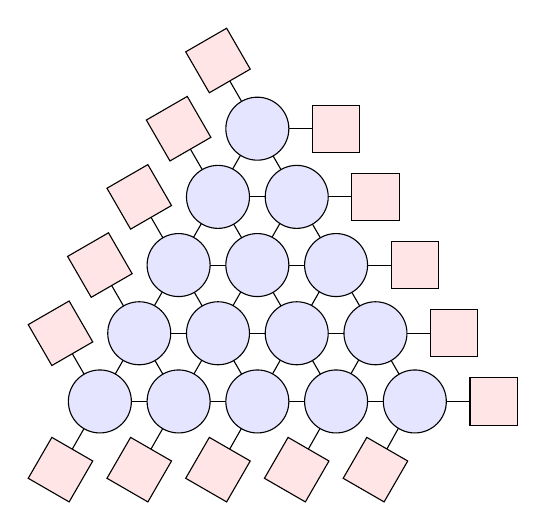
\begin{tikzpicture}
    \def\r{0.3}

    \foreach \x/\y in {1/4, 2/3, 3/2, 4/1, 5/0} {
      \draw (0.5 * \y, {\y * sqrt(3)/2})--(\x + 0.5 * \y, {\y * sqrt(3)/2});
      \draw[fill=red!10]
        (\x - \r + 0.5 * \y, {\y * sqrt(3)/2 - \r}) rectangle
        (\x + \r + 0.5 * \y, {\y * sqrt(3)/2 + \r});
    }

    \foreach \x/\y in {0/-1, 1/-1, 2/-1, 3/-1, 4/-1} {
      % \draw[<-] (0.75 + \x + 0.5 * \y, {\y * sqrt(3)/2})--(1.1 + \x + 0.5 * \y, {\y * sqrt(3)/2});
      \draw (0.5 * \x + 2, {3.5-\x* sqrt(3)/2})--(\x + 0.5 * \y, {\y * sqrt(3)/2});
      \draw[fill=red!10, rotate around={60:({\x + 0.5 * \y}, {\y * sqrt(3)/2})}]
        (\x - \r + 0.5 * \y, {\y * sqrt(3)/2 - \r}) rectangle
        (\x + \r + 0.5 * \y, {\y * sqrt(3)/2 + \r});
    }

    \foreach \x/\y in {-1/1, -1/2, -1/3, -1/4, -1/5} {
      \draw (\y - 1, 0)--(\x + 0.5 * \y, {\y * sqrt(3)/2});
      \draw[fill=red!10, rotate around={-60:({\x + 0.5 * \y}, {\y * sqrt(3)/2})}]
        (\x - \r + 0.5 * \y, {\y * sqrt(3)/2 - \r}) rectangle
        (\x + \r + 0.5 * \y, {\y * sqrt(3)/2 + \r});
    }
    \foreach \x/\y in {
      0/0, 0/1, 0/2, 0/3, 0/4,
      1/0, 1/1, 1/2, 1/3,
      2/0, 2/1, 2/2,
      3/0, 3/1,
      4/0} {
      \draw[fill=blue!10] (\x + 0.5 * \y, {\y * sqrt(3)/2}) circle (0.4cm);
    }
  \end{tikzpicture}
  \caption{
    Examples of all known classes of polygonal chains of length $4$.
  }
\end{figure}
\begin{question}
  Which player has a winning strategy?
\end{question}

\begin{related}
  \item Does perfect play result in a tie?
  \item How many turns are required under perfect play
    where the winner attempts to win in as few turns as possible, and the
    loser attempts to lose in as many turns as possible?
  \item What if multiple markers can be placed in each row?
  \item How does this generalize to other geometries?
  \item The square analog is essentially the same game under action of the
    torus. Is there an action (besides rotation) that behaves similarly?
\end{related}
\begin{references}
  \item Problem 49.
\end{references}
\end{document}
